\documentclass{standalone}
\usepackage{tikz}
\usetikzlibrary{patterns, positioning}
\usepackage[sfdefault]{ClearSans} %% option 'sfdefault' activates Clear Sans as the default text font
\usepackage[T1]{fontenc}

\begin{document}
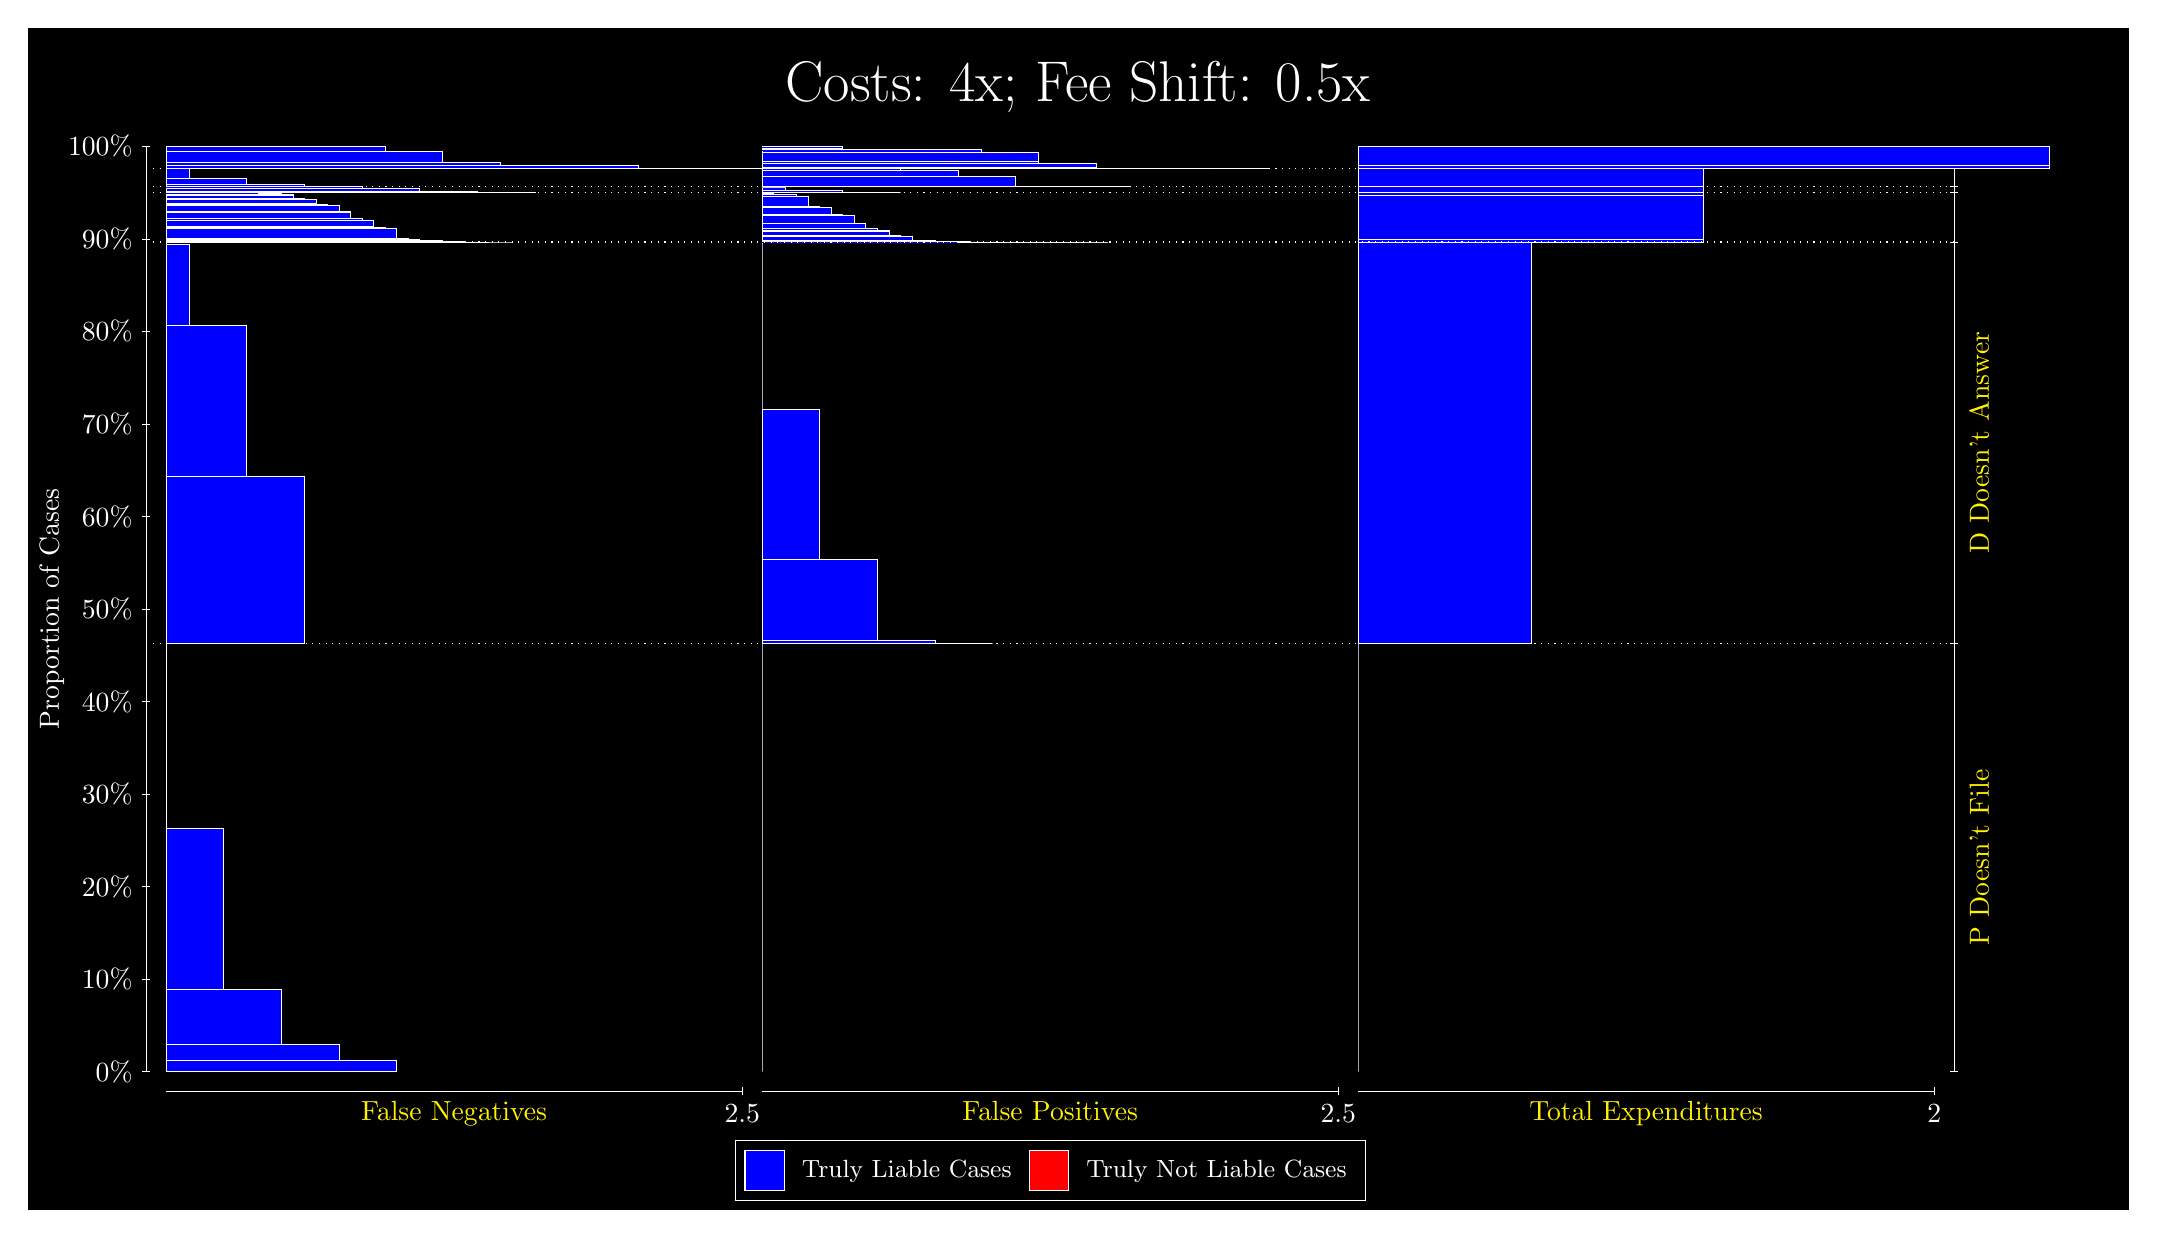
\begin{tikzpicture}
\draw[fill=black] (0,0) rectangle (26.667,15);
\draw[text=white] (0,13.5) rectangle (26.667,15) node[midway] {\huge Costs: 4x; Fee Shift: 0.5x};
\draw[white, very thin] (1.5,1.75) -- (1.5,13.5);
\node[rotate=90, text=white, anchor=center] at (0.3, 7.625) {Proportion of Cases};
\draw[white, very thin] (1.45,1.75) -- (1.55,1.75);
\node[text=white, anchor=east] at (1.45, 1.75) {0\%};
\draw[white, very thin] (1.45,2.925) -- (1.55,2.925);
\node[text=white, anchor=east] at (1.45, 2.925) {10\%};
\draw[white, very thin] (1.45,4.1) -- (1.55,4.1);
\node[text=white, anchor=east] at (1.45, 4.1) {20\%};
\draw[white, very thin] (1.45,5.275) -- (1.55,5.275);
\node[text=white, anchor=east] at (1.45, 5.275) {30\%};
\draw[white, very thin] (1.45,6.45) -- (1.55,6.45);
\node[text=white, anchor=east] at (1.45, 6.45) {40\%};
\draw[white, very thin] (1.45,7.625) -- (1.55,7.625);
\node[text=white, anchor=east] at (1.45, 7.625) {50\%};
\draw[white, very thin] (1.45,8.8) -- (1.55,8.8);
\node[text=white, anchor=east] at (1.45, 8.8) {60\%};
\draw[white, very thin] (1.45,9.975) -- (1.55,9.975);
\node[text=white, anchor=east] at (1.45, 9.975) {70\%};
\draw[white, very thin] (1.45,11.15) -- (1.55,11.15);
\node[text=white, anchor=east] at (1.45, 11.15) {80\%};
\draw[white, very thin] (1.45,12.325) -- (1.55,12.325);
\node[text=white, anchor=east] at (1.45, 12.325) {90\%};
\draw[white, very thin] (1.45,13.5) -- (1.55,13.5);
\node[text=white, anchor=east] at (1.45, 13.5) {100\%};

\draw[white, very thin] (24.457,1.75) -- (24.457,13.5);
\draw[white, very thin] (24.407,1.75) -- (24.507,1.75);
\node[anchor=west] at (24.407, 1.75) {};
\draw[white, very thin] (24.407,7.1882) -- (24.507,7.1882);
\node[anchor=west] at (24.407, 7.1882) {};
\draw[white, very thin] (24.407,12.285) -- (24.507,12.285);
\node[anchor=west] at (24.407, 12.285) {};
\draw[white, very thin] (24.407,12.917) -- (24.507,12.917);
\node[anchor=west] at (24.407, 12.917) {};
\draw[white, very thin] (24.407,12.989) -- (24.507,12.989);
\node[anchor=west] at (24.407, 12.989) {};
\draw[white, very thin] (24.407,13.222) -- (24.507,13.222);
\node[anchor=west] at (24.407, 13.222) {};
\draw[white, very thin] (24.407,13.5) -- (24.507,13.5);
\node[anchor=west] at (24.407, 13.5) {};

\draw[white, very thin, fill=blue] (1.75,1.75) rectangle (4.6775,1.8962);
\draw[white, very thin, fill=blue] (1.75,1.8962) rectangle (3.9457,2.0924);
\draw[white, very thin, fill=blue] (1.75,2.0924) rectangle (3.2138,2.7939);
\draw[white, very thin, fill=blue] (1.75,2.7939) rectangle (2.4819,4.8412);
\draw[white, very thin, fill=red] (1.75,4.8412) rectangle (1.75,4.8412);
\draw[white, very thin, fill=blue] (1.75,4.8412) rectangle (1.75,7.1882);
\draw[white, very thin, fill=blue] (1.75,7.1882) rectangle (3.5065,9.3075);
\draw[white, very thin, fill=blue] (1.75,9.3075) rectangle (2.7746,11.221);
\draw[white, very thin, fill=blue] (1.75,11.221) rectangle (2.0428,12.251);
\draw[white, very thin, fill=red] (1.75,12.251) rectangle (1.75,12.251);
\draw[white, very thin, fill=blue] (1.75,12.251) rectangle (1.75,12.285);
\draw[white, very thin, fill=blue] (1.75,12.285) rectangle (6.1413,12.285);
\draw[white, very thin, fill=blue] (1.75,12.285) rectangle (5.8486,12.286);
\draw[white, very thin, fill=blue] (1.75,12.286) rectangle (5.5558,12.288);
\draw[white, very thin, fill=blue] (1.75,12.288) rectangle (5.4094,12.3);
\draw[white, very thin, fill=blue] (1.75,12.3) rectangle (5.2631,12.302);
\draw[white, very thin, fill=blue] (1.75,12.302) rectangle (5.1167,12.312);
\draw[white, very thin, fill=blue] (1.75,12.312) rectangle (4.9703,12.316);
\draw[white, very thin, fill=blue] (1.75,12.316) rectangle (4.8239,12.337);
\draw[white, very thin, fill=blue] (1.75,12.337) rectangle (4.6775,12.462);
\draw[white, very thin, fill=blue] (1.75,12.462) rectangle (4.5312,12.475);
\draw[white, very thin, fill=blue] (1.75,12.475) rectangle (4.3848,12.482);
\draw[white, very thin, fill=blue] (1.75,12.482) rectangle (4.3848,12.566);
\draw[white, very thin, fill=blue] (1.75,12.566) rectangle (4.2384,12.581);
\draw[white, very thin, fill=blue] (1.75,12.581) rectangle (4.092,12.667);
\draw[white, very thin, fill=blue] (1.75,12.667) rectangle (4.092,12.673);
\draw[white, very thin, fill=blue] (1.75,12.673) rectangle (3.9457,12.749);
\draw[white, very thin, fill=blue] (1.75,12.749) rectangle (3.7993,12.769);
\draw[white, very thin, fill=blue] (1.75,12.769) rectangle (3.6529,12.781);
\draw[white, very thin, fill=blue] (1.75,12.781) rectangle (3.6529,12.828);
\draw[white, very thin, fill=blue] (1.75,12.828) rectangle (3.5065,12.842);
\draw[white, very thin, fill=blue] (1.75,12.842) rectangle (3.3602,12.884);
\draw[white, very thin, fill=blue] (1.75,12.884) rectangle (3.3602,12.892);
\draw[white, very thin, fill=blue] (1.75,12.892) rectangle (3.2138,12.901);
\draw[white, very thin, fill=blue] (1.75,12.901) rectangle (3.0674,12.901);
\draw[white, very thin, fill=blue] (1.75,12.901) rectangle (3.0674,12.908);
\draw[white, very thin, fill=blue] (1.75,12.908) rectangle (2.921,12.911);
\draw[white, very thin, fill=blue] (1.75,12.911) rectangle (2.921,12.912);
\draw[white, very thin, fill=blue] (1.75,12.912) rectangle (2.7746,12.912);
\draw[white, very thin, fill=blue] (1.75,12.912) rectangle (2.6283,12.913);
\draw[white, very thin, fill=blue] (1.75,12.913) rectangle (2.6283,12.915);
\draw[white, very thin, fill=blue] (1.75,12.915) rectangle (2.4819,12.915);
\draw[white, very thin, fill=blue] (1.75,12.915) rectangle (2.3355,12.915);
\draw[white, very thin, fill=blue] (1.75,12.915) rectangle (2.3355,12.917);
\draw[white, very thin, fill=blue] (1.75,12.917) rectangle (2.1891,12.917);
\draw[white, very thin, fill=blue] (1.75,12.917) rectangle (2.0428,12.917);
\draw[white, very thin, fill=blue] (1.75,12.917) rectangle (1.8964,12.917);
\draw[white, very thin, fill=red] (1.75,12.917) rectangle (1.75,12.917);
\draw[white, very thin, fill=blue] (1.75,12.917) rectangle (1.75,12.917);
\draw[white, very thin, fill=blue] (1.75,12.917) rectangle (6.4341,12.918);
\draw[white, very thin, fill=blue] (1.75,12.918) rectangle (5.7022,12.923);
\draw[white, very thin, fill=blue] (1.75,12.923) rectangle (4.9703,12.962);
\draw[white, very thin, fill=blue] (1.75,12.962) rectangle (4.2384,12.988);
\draw[white, very thin, fill=blue] (1.75,12.988) rectangle (3.5065,12.989);
\draw[white, very thin, fill=red] (1.75,12.989) rectangle (1.75,12.989);
\draw[white, very thin, fill=blue] (1.75,12.989) rectangle (3.5065,13.012);
\draw[white, very thin, fill=blue] (1.75,13.012) rectangle (2.7746,13.096);
\draw[white, very thin, fill=blue] (1.75,13.096) rectangle (2.0428,13.218);
\draw[white, very thin, fill=red] (1.75,13.218) rectangle (1.75,13.218);
\draw[white, very thin, fill=blue] (1.75,13.218) rectangle (1.75,13.222);
\draw[white, very thin, fill=blue] (1.75,13.222) rectangle (9.9471,13.222);
\draw[white, very thin, fill=blue] (1.75,13.222) rectangle (9.2152,13.222);
\draw[white, very thin, fill=blue] (1.75,13.222) rectangle (8.4834,13.226);
\draw[white, very thin, fill=blue] (1.75,13.226) rectangle (7.7515,13.255);
\draw[white, very thin, fill=blue] (1.75,13.255) rectangle (7.4587,13.255);
\draw[white, very thin, fill=blue] (1.75,13.255) rectangle (7.0196,13.264);
\draw[white, very thin, fill=blue] (1.75,13.264) rectangle (6.7268,13.265);
\draw[white, very thin, fill=blue] (1.75,13.265) rectangle (6.2877,13.265);
\draw[white, very thin, fill=blue] (1.75,13.265) rectangle (5.9949,13.302);
\draw[white, very thin, fill=blue] (1.75,13.302) rectangle (5.5558,13.302);
\draw[white, very thin, fill=blue] (1.75,13.302) rectangle (5.2631,13.437);
\draw[white, very thin, fill=blue] (1.75,13.437) rectangle (4.5312,13.495);
\draw[white, very thin, fill=blue] (1.75,13.495) rectangle (3.7993,13.5);
\draw[white, very thin, fill=blue] (1.75,13.5) rectangle (3.0674,13.5);
\draw[white, very thin, fill=blue] (1.75,13.5) rectangle (2.3355,13.5);
\draw[white, very thin, fill=red] (1.75,13.5) rectangle (1.75,13.5);
\draw[white, very thin, fill=red] (9.3189,1.75) rectangle (9.3189,1.75);
\draw[white, very thin, fill=blue] (9.3189,1.75) rectangle (9.3189,7.1882);
\draw[white, very thin, fill=red] (9.3189,7.1882) rectangle (12.246,7.1882);
\draw[white, very thin, fill=blue] (9.3189,7.1882) rectangle (12.246,7.1882);
\draw[white, very thin, fill=blue] (9.3189,7.1882) rectangle (11.515,7.2221);
\draw[white, very thin, fill=blue] (9.3189,7.2221) rectangle (10.783,8.2519);
\draw[white, very thin, fill=blue] (9.3189,8.2519) rectangle (10.051,10.165);
\draw[white, very thin, fill=blue] (9.3189,10.165) rectangle (9.3189,12.285);
\draw[white, very thin, fill=red] (9.3189,12.285) rectangle (13.71,12.285);
\draw[white, very thin, fill=blue] (9.3189,12.285) rectangle (13.71,12.285);
\draw[white, very thin, fill=red] (9.3189,12.285) rectangle (13.417,12.285);
\draw[white, very thin, fill=blue] (9.3189,12.285) rectangle (13.417,12.285);
\draw[white, very thin, fill=red] (9.3189,12.285) rectangle (13.125,12.285);
\draw[white, very thin, fill=blue] (9.3189,12.285) rectangle (13.125,12.285);
\draw[white, very thin, fill=blue] (9.3189,12.285) rectangle (12.978,12.285);
\draw[white, very thin, fill=red] (9.3189,12.285) rectangle (12.832,12.285);
\draw[white, very thin, fill=blue] (9.3189,12.285) rectangle (12.832,12.285);
\draw[white, very thin, fill=blue] (9.3189,12.285) rectangle (12.686,12.285);
\draw[white, very thin, fill=red] (9.3189,12.285) rectangle (12.539,12.285);
\draw[white, very thin, fill=blue] (9.3189,12.285) rectangle (12.539,12.285);
\draw[white, very thin, fill=blue] (9.3189,12.285) rectangle (12.393,12.285);
\draw[white, very thin, fill=red] (9.3189,12.285) rectangle (12.246,12.285);
\draw[white, very thin, fill=blue] (9.3189,12.285) rectangle (12.246,12.286);
\draw[white, very thin, fill=blue] (9.3189,12.286) rectangle (12.1,12.286);
\draw[white, very thin, fill=red] (9.3189,12.286) rectangle (11.954,12.286);
\draw[white, very thin, fill=blue] (9.3189,12.286) rectangle (11.954,12.289);
\draw[white, very thin, fill=blue] (9.3189,12.289) rectangle (11.807,12.29);
\draw[white, very thin, fill=red] (9.3189,12.29) rectangle (11.661,12.29);
\draw[white, very thin, fill=blue] (9.3189,12.29) rectangle (11.661,12.29);
\draw[white, very thin, fill=blue] (9.3189,12.29) rectangle (11.661,12.294);
\draw[white, very thin, fill=blue] (9.3189,12.294) rectangle (11.515,12.301);
\draw[white, very thin, fill=red] (9.3189,12.301) rectangle (11.368,12.301);
\draw[white, very thin, fill=blue] (9.3189,12.301) rectangle (11.368,12.309);
\draw[white, very thin, fill=blue] (9.3189,12.309) rectangle (11.222,12.359);
\draw[white, very thin, fill=blue] (9.3189,12.359) rectangle (11.075,12.373);
\draw[white, very thin, fill=blue] (9.3189,12.373) rectangle (10.929,12.421);
\draw[white, very thin, fill=blue] (9.3189,12.421) rectangle (10.929,12.432);
\draw[white, very thin, fill=blue] (9.3189,12.432) rectangle (10.783,12.453);
\draw[white, very thin, fill=blue] (9.3189,12.453) rectangle (10.636,12.529);
\draw[white, very thin, fill=blue] (9.3189,12.529) rectangle (10.49,12.621);
\draw[white, very thin, fill=blue] (9.3189,12.621) rectangle (10.344,12.635);
\draw[white, very thin, fill=blue] (9.3189,12.635) rectangle (10.197,12.72);
\draw[white, very thin, fill=blue] (9.3189,12.72) rectangle (10.197,12.727);
\draw[white, very thin, fill=blue] (9.3189,12.727) rectangle (10.051,12.739);
\draw[white, very thin, fill=blue] (9.3189,12.739) rectangle (9.9044,12.865);
\draw[white, very thin, fill=blue] (9.3189,12.865) rectangle (9.758,12.886);
\draw[white, very thin, fill=blue] (9.3189,12.886) rectangle (9.6116,12.89);
\draw[white, very thin, fill=blue] (9.3189,12.89) rectangle (9.4652,12.9);
\draw[white, very thin, fill=blue] (9.3189,12.9) rectangle (9.3189,12.917);
\draw[white, very thin, fill=red] (9.3189,12.917) rectangle (11.075,12.917);
\draw[white, very thin, fill=blue] (9.3189,12.917) rectangle (11.075,12.917);
\draw[white, very thin, fill=blue] (9.3189,12.917) rectangle (10.344,12.944);
\draw[white, very thin, fill=blue] (9.3189,12.944) rectangle (9.6116,12.982);
\draw[white, very thin, fill=blue] (9.3189,12.982) rectangle (9.3189,12.989);
\draw[white, very thin, fill=red] (9.3189,12.989) rectangle (14.003,12.989);
\draw[white, very thin, fill=blue] (9.3189,12.989) rectangle (14.003,12.989);
\draw[white, very thin, fill=blue] (9.3189,12.989) rectangle (13.271,12.993);
\draw[white, very thin, fill=blue] (9.3189,12.993) rectangle (12.539,13.115);
\draw[white, very thin, fill=blue] (9.3189,13.115) rectangle (11.807,13.199);
\draw[white, very thin, fill=blue] (9.3189,13.199) rectangle (11.075,13.222);
\draw[white, very thin, fill=red] (9.3189,13.222) rectangle (15.759,13.222);
\draw[white, very thin, fill=blue] (9.3189,13.222) rectangle (15.759,13.222);
\draw[white, very thin, fill=blue] (9.3189,13.222) rectangle (15.028,13.222);
\draw[white, very thin, fill=red] (9.3189,13.222) rectangle (15.028,13.222);
\draw[white, very thin, fill=blue] (9.3189,13.222) rectangle (15.028,13.222);
\draw[white, very thin, fill=blue] (9.3189,13.222) rectangle (14.296,13.225);
\draw[white, very thin, fill=red] (9.3189,13.225) rectangle (14.296,13.225);
\draw[white, very thin, fill=blue] (9.3189,13.225) rectangle (14.296,13.227);
\draw[white, very thin, fill=blue] (9.3189,13.227) rectangle (13.564,13.237);
\draw[white, very thin, fill=red] (9.3189,13.237) rectangle (13.564,13.237);
\draw[white, very thin, fill=blue] (9.3189,13.237) rectangle (13.564,13.285);
\draw[white, very thin, fill=blue] (9.3189,13.285) rectangle (12.832,13.304);
\draw[white, very thin, fill=blue] (9.3189,13.304) rectangle (12.832,13.421);
\draw[white, very thin, fill=red] (9.3189,13.421) rectangle (12.539,13.421);
\draw[white, very thin, fill=blue] (9.3189,13.421) rectangle (12.539,13.421);
\draw[white, very thin, fill=blue] (9.3189,13.421) rectangle (12.1,13.458);
\draw[white, very thin, fill=blue] (9.3189,13.458) rectangle (11.807,13.458);
\draw[white, very thin, fill=red] (9.3189,13.458) rectangle (11.807,13.458);
\draw[white, very thin, fill=blue] (9.3189,13.458) rectangle (11.807,13.458);
\draw[white, very thin, fill=blue] (9.3189,13.458) rectangle (11.368,13.459);
\draw[white, very thin, fill=blue] (9.3189,13.459) rectangle (11.075,13.46);
\draw[white, very thin, fill=red] (9.3189,13.46) rectangle (11.075,13.46);
\draw[white, very thin, fill=blue] (9.3189,13.46) rectangle (11.075,13.467);
\draw[white, very thin, fill=blue] (9.3189,13.467) rectangle (10.636,13.467);
\draw[white, very thin, fill=blue] (9.3189,13.467) rectangle (10.344,13.47);
\draw[white, very thin, fill=blue] (9.3189,13.47) rectangle (10.344,13.496);
\draw[white, very thin, fill=blue] (9.3189,13.496) rectangle (9.6116,13.497);
\draw[white, very thin, fill=blue] (9.3189,13.497) rectangle (9.6116,13.5);
\draw[white, very thin, fill=blue] (9.3189,13.5) rectangle (9.3189,13.5);
\draw[white, very thin, fill=red] (16.888,1.75) rectangle (16.888,1.75);
\draw[white, very thin, fill=blue] (16.888,1.75) rectangle (16.888,7.1882);
\draw[white, very thin, fill=red] (16.888,7.1882) rectangle (19.083,7.1882);
\draw[white, very thin, fill=blue] (16.888,7.1882) rectangle (19.083,12.285);
\draw[white, very thin, fill=red] (16.888,12.285) rectangle (21.279,12.285);
\draw[white, very thin, fill=blue] (16.888,12.285) rectangle (21.279,12.318);
\draw[white, very thin, fill=red] (16.888,12.318) rectangle (21.279,12.318);
\draw[white, very thin, fill=blue] (16.888,12.318) rectangle (21.279,12.879);
\draw[white, very thin, fill=red] (16.888,12.879) rectangle (21.279,12.879);
\draw[white, very thin, fill=blue] (16.888,12.879) rectangle (21.279,12.917);
\draw[white, very thin, fill=red] (16.888,12.917) rectangle (21.279,12.917);
\draw[white, very thin, fill=blue] (16.888,12.917) rectangle (21.279,12.989);
\draw[white, very thin, fill=red] (16.888,12.989) rectangle (21.279,12.989);
\draw[white, very thin, fill=blue] (16.888,12.989) rectangle (21.279,13.222);
\draw[white, very thin, fill=red] (16.888,13.222) rectangle (25.67,13.222);
\draw[white, very thin, fill=blue] (16.888,13.222) rectangle (25.67,13.254);
\draw[white, very thin, fill=red] (16.888,13.254) rectangle (25.67,13.254);
\draw[white, very thin, fill=blue] (16.888,13.254) rectangle (25.67,13.5);
\draw[white, dotted] (1.5,7.1882) -- (24.457,7.1882);
\draw[white, dotted] (1.5,12.285) -- (24.457,12.285);
\draw[white, dotted] (1.5,12.917) -- (24.457,12.917);
\draw[white, dotted] (1.5,12.989) -- (24.457,12.989);
\draw[white, dotted] (1.5,13.222) -- (24.457,13.222);
\draw[white, very thin] (1.75,1.5) -- (9.0689,1.5);
\node[text=yellow, anchor=north] at (5.4094, 1.5) {False Negatives};
\draw[white, very thin] (9.0689,1.45) -- (9.0689,1.55);
\node[text=white, anchor=north] at (9.0689, 1.45) {2.5};

\draw[white, very thin] (9.3189,1.5) -- (16.638,1.5);
\node[text=yellow, anchor=north] at (12.978, 1.5) {False Positives};
\draw[white, very thin] (16.638,1.45) -- (16.638,1.55);
\node[text=white, anchor=north] at (16.638, 1.45) {2.5};

\draw[white, very thin] (16.888,1.5) -- (24.207,1.5);
\node[text=yellow, anchor=north] at (20.547, 1.5) {Total Expenditures};
\draw[white, very thin] (24.207,1.45) -- (24.207,1.55);
\node[text=white, anchor=north] at (24.207, 1.45) {2};

\node[text=yellow, centered, rotate=90] at (24.777, 4.4691) {P Doesn't File};
\node[text=yellow, centered, rotate=90] at (24.777, 9.7364) {D Doesn't Answer};





\draw (12.978300999999998,1.5) node[draw=none] (baseCoordinate) {};
\begin{scope}[align=center]
        \matrix[scale=0.5, draw=white, below=0.5cm of baseCoordinate, nodes={draw}, column sep=0.1cm]{
            \node[rectangle, draw, minimum width=0.5cm, minimum height=0.5cm, fill=blue] {}; &
            \node[draw=none, font=\small, text=white] (B) {Truly Liable Cases}; &
            \node[rectangle, draw, minimum width=0.5cm, minimum height=0.5cm, fill=red] {}; &
            \node[draw=none, font=\small, text=white] (B) {Truly Not Liable Cases}; \\
            };
\end{scope}

\end{tikzpicture}
\end{document}